% ----------------------------------------------------
% Validation and Simulation
% ----------------------------------------------------
\documentclass[class=report,11pt,crop=false]{standalone}
\input{../Style/ChapterStyle.tex}
\makenoidxglossaries

\newacronym{fm}{FM}{frequency modulation}
\newacronym{lora}{LoRa}{Long Range}
\newacronym{iot}{IOT}{Internet of Things}
\newacronym{fsk}{FSK}{Frequency Shift Keying}
\newacronym{chirp}{CHIRP}{Compressed High Intensity Radar Pulse}
\newacronym{atps}{ATPs}{Acceptance Test Protocols}
\newacronym{hal}{HAL}{Hardware Abstraction Layer}
\newacronym{oled}{OLED}{Organic Light Emitting Diode}
\newacronym{rssi}{RSSI}{Received Signal Strength Index}
\newacronym{uart}{UART}{Universal Asynchronous Receive and Transmit}
\newacronym{usb}{USB}{Universal Serial Bus}
\newacronym{css}{CSS}{Chirp Spread Spectrum}
\newacronym{i2c}{I2C}{Inter-Integrated Circuit}
\newacronym{spi}{SPI}{Serial Peripheral Interface}
\newacronym{gps}{GPS}{Global Positioning System}
\newacronym{nmea}{NMEA}{National Marine Electronics Association}
\newacronym{mac}{MAC}{Media Access Control}
\newacronym{sf}{SF}{Spreading Factor}
\newacronym{arr}{ARR}{Auto Reload Register}
\newacronym{sdr}{SDR}{Software Defined Radio}
\newacronym{pcb}{PCB}{Printed Circuit Board}
\newacronym{fdm}{FDM}{Frequency Division Multiplexing}


\newacronym{radar}{RADAR}{Radio Detection and Ranging}
\newacronym{ofdm}{OFDM}{Orthogonal Frequency Division Multiplexing}
\newacronym{tdm}{TDM}{Time Division Multiplexing}
\newacronym{tdma}{TDMA}{Time Division Multiple Access}
\newacronym{att}{AT\&T}{American Telephone and Telegraph Company}
\newacronym{usrp}{USRP}{Universal Software Radio Peripheral}
\newacronym{uct}{UCT}{University of Cape Town}


\begin{document}
% ----------------------------------------------------
\chapter{Validation and Simulation \label{ch:validationandsimulation}}
In order to test that the overall system was working, various tests were performed in order to validate that the many modules and sub-modules were working in a manner that was acceptable. As well as the tests performed on the system to determine the validity of the modules and sub-modules, certain simulations were performed in order to determine certain performance characteristics of the system before actual tests were performed.
\section{Validation}
The thought process that went into validating each part of the individual modules is outlined in the following sections.
\subsection{Transmitter Validation}
\subsubsection{Power Module}
The power module was deemed to be a successful implementation of the circuitry since it was able to easily supply the entire transmitter circuit. The output of the power module was measured to be 5V, which is the correct voltage that it should be outputting, and which can supply the STM32F411 microcontroller. The microcontroller then took care of all the devices which required 3.3V.
\subsubsection{Microcontroller}
The microcontroller was seen to be able to communicate with all the sensor modules, process the data, and handle the different modes of operation of the system. It was therefore decided that the microcontroller was correctly implemented and could be validated to be working.
\subsubsection{Sensor Modules}
The sensor modules that formed part of the transmission circuit were all deemed to be successfully implemented. Seen below in listing \ref{lst:sensormodulevalidation} is a sample output of a packet created for the transmission circuit. 
\begin{lstlisting}[caption={Sample Data from Sensor Modules}, label={lst:sensormodulevalidation}]
"14:48:12|(-335745239,182936654)|102416.44|18.87|44.89|-90.473"
\end{lstlisting}
This recording was taken at 16:48 South African time (UTC + 02:00). Therefore, one can see that the time stamp is correct, seeing as it is UTC + 00:00. If the same process that is followed in section \ref{sec:contructionofdatapacket} is followed on the GPS data, the following GPS coordinates are produced, (-33.95753983,18.48944233). These coordinates correspond to the following location shown in figure \ref{fig:gpsvalidation} below. The red pin corresponds to the GPS data from the transmitter module, and the blue dot is the actual location of my laptop according to Google Maps.

\begin{figure}[H]
    \centering
    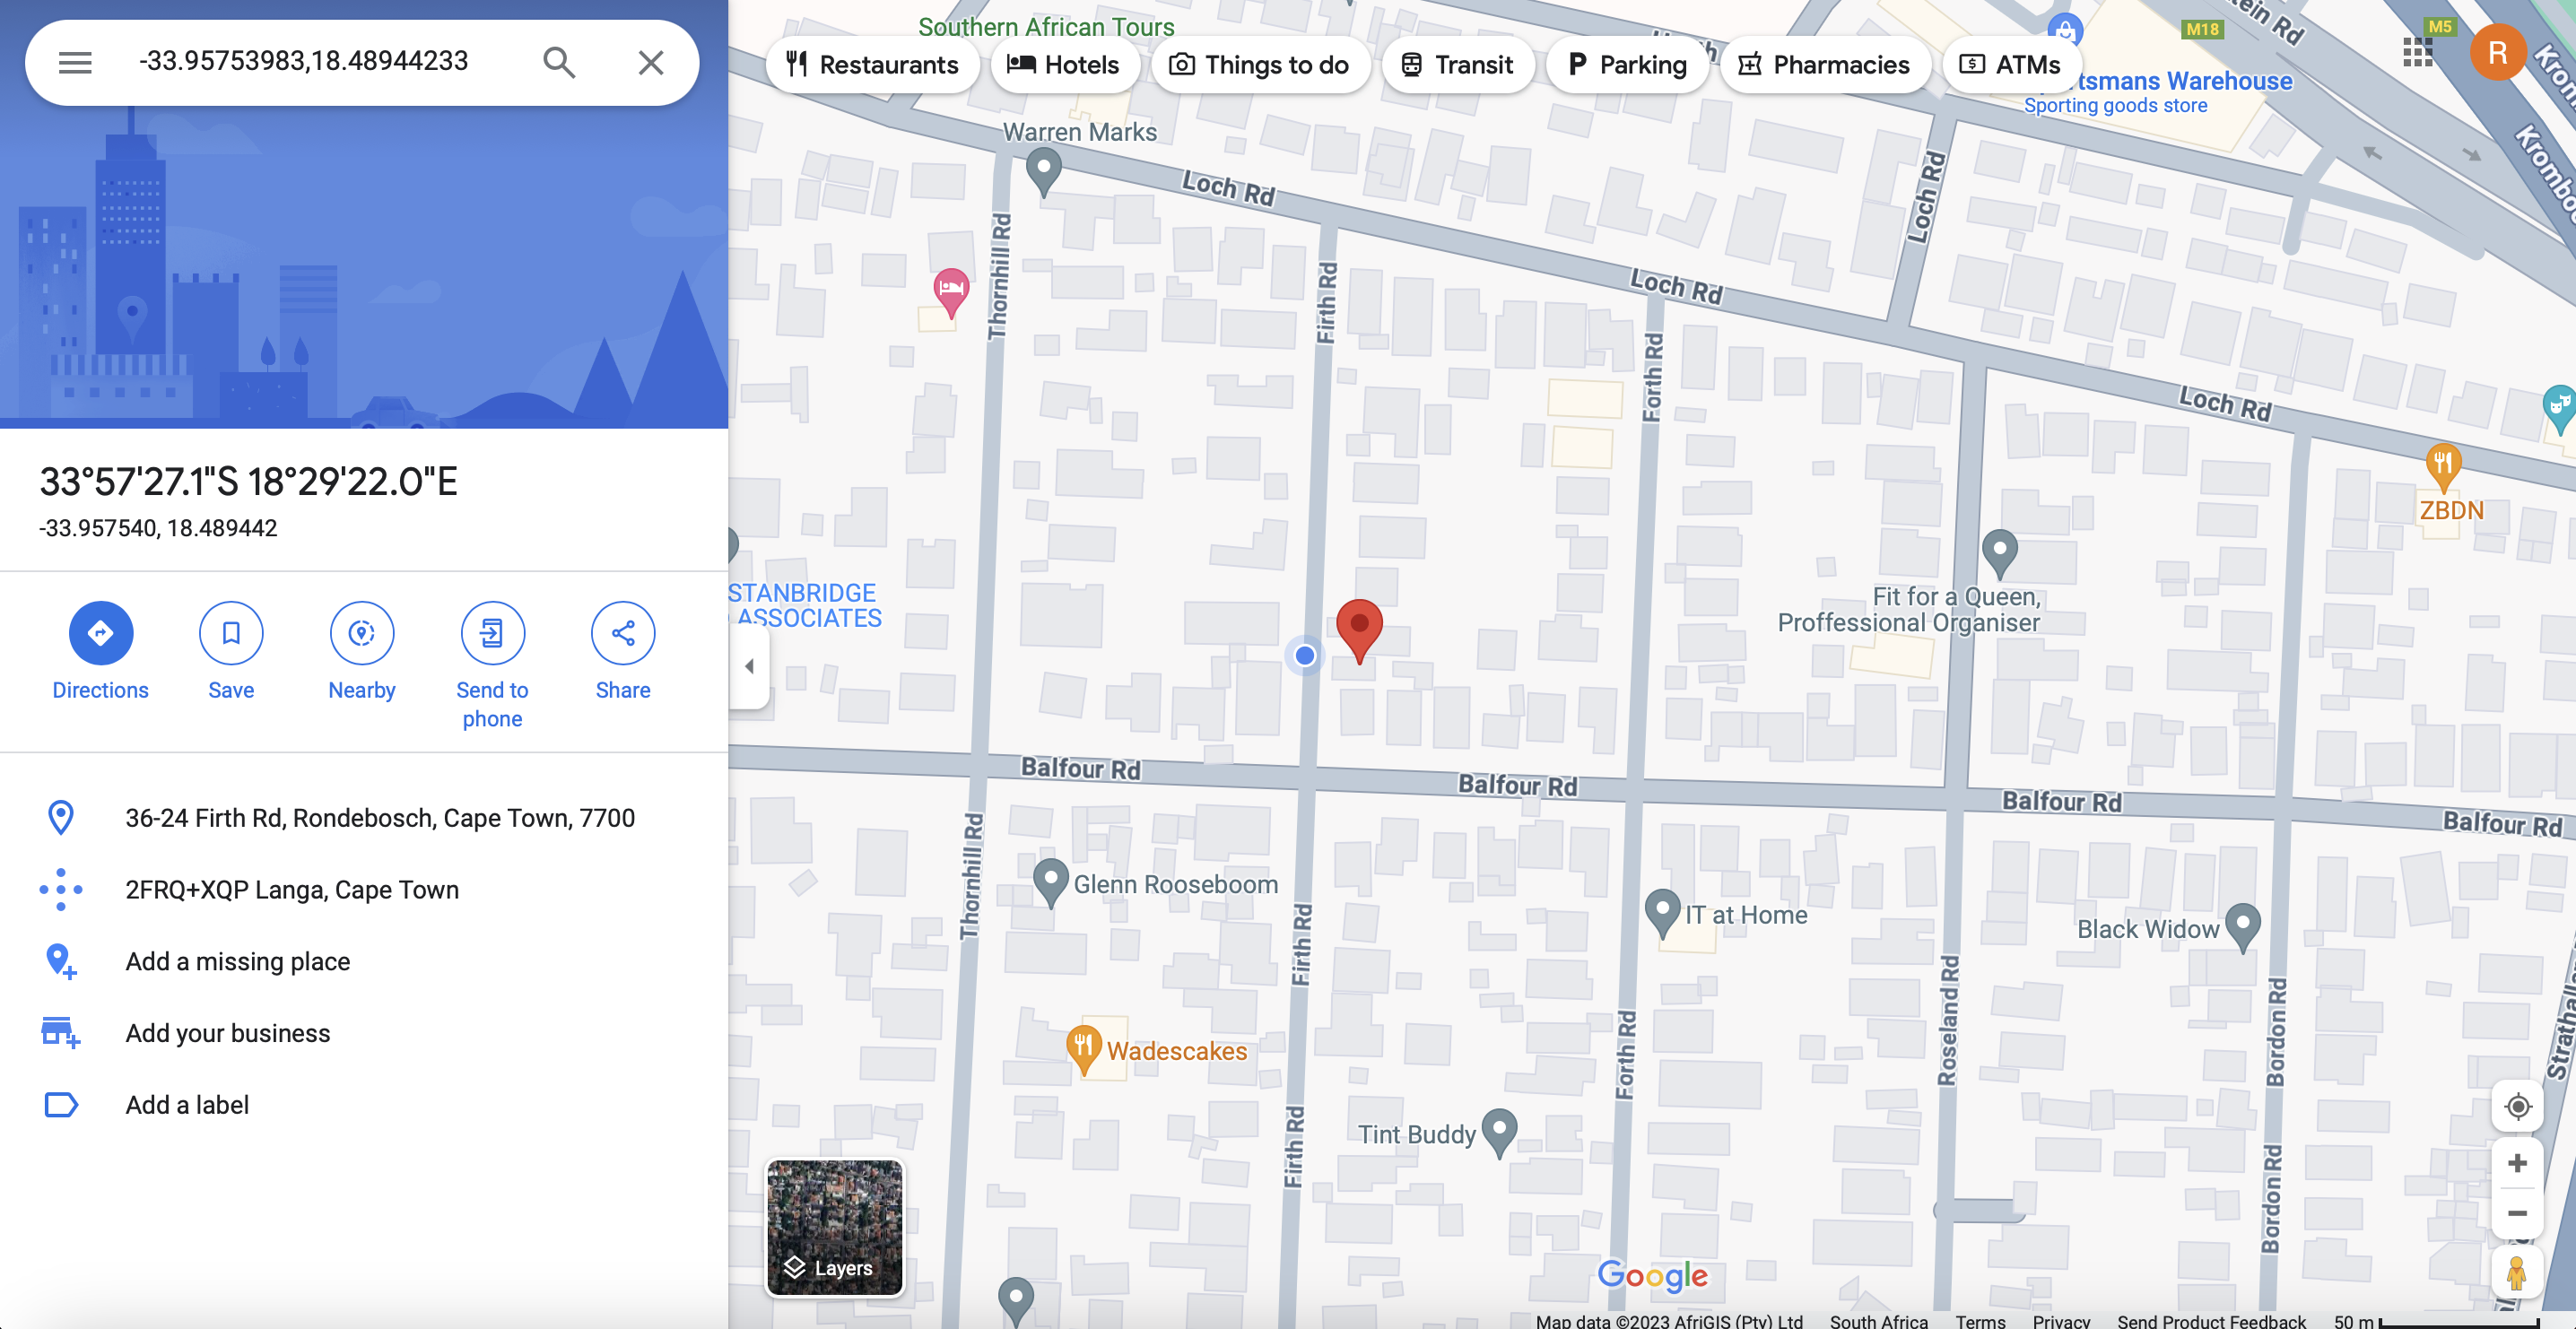
\includegraphics[width=0.7\linewidth]{../Images/gpsValidation.png}
    \caption{GPS Data Validation}
    \label{fig:gpsvalidation}
\end{figure}

It can be seen that the GPS data is therefore correct. The pressure, temperature, and humidity data were compared with current readings from the Apple Weather application and were all within roughly 10\% of the Apple Weather readings. It was therefore deemed that the sensor modules were operating correctly. A more accurate validation could not be performed due to the lack of highly accurate atmospheric measurement devices available to me at the time. Lastly, the altitude reading. Since the altitude reading was a calculation based on the barometric equation (equation \ref{eq:barometricformula}), it can sometimes give inaccurate results based on how far off the true sea level pressure is at a location where the pressure is being measured. This issue can be mitigated by using the altitude measurement from the GPS module, however, this falls into the category of future work and was not actively developed for this project.

\subsubsection{LoRa module and Display and Control Module}
The display and control module was validated through a test performed where the various modes of operation were cycled through and it was observed whether or not the OLED display updated with the correct mode of operation, and whether the LoRa settings updated corresponding to the correct mode. To check whether the LoRa module was properly getting its parameters updated each time a mode was changed, a \gls{sdr} was utilised to check whether the LoRa settings were being changed, and on a broader level whether the LoRa transmissions were working in the first place. A snapshot of the output of the SDR for a LoRa transmission at a spreading factor of 12, and a bandwidth of 500kHz can be seen in figure \ref{fig:loravalidationwithsdr} below. It was determined that the mode changes did indeed change the parameters of the Lora transmission, in that increasing the spreading factor increased the length of the transmissions, and increasing the bandwidth increased the bandwidth over which the chirps occurred. Then from a broad perspective, it was noted that the actual LoRa transmission was indeed working. In the below figure, one can make out the discontinuities that were mentioned in chapter \ref{ch:Literature} that are so unique to a LoRa transmission.

\begin{figure}[H]
    \centering
    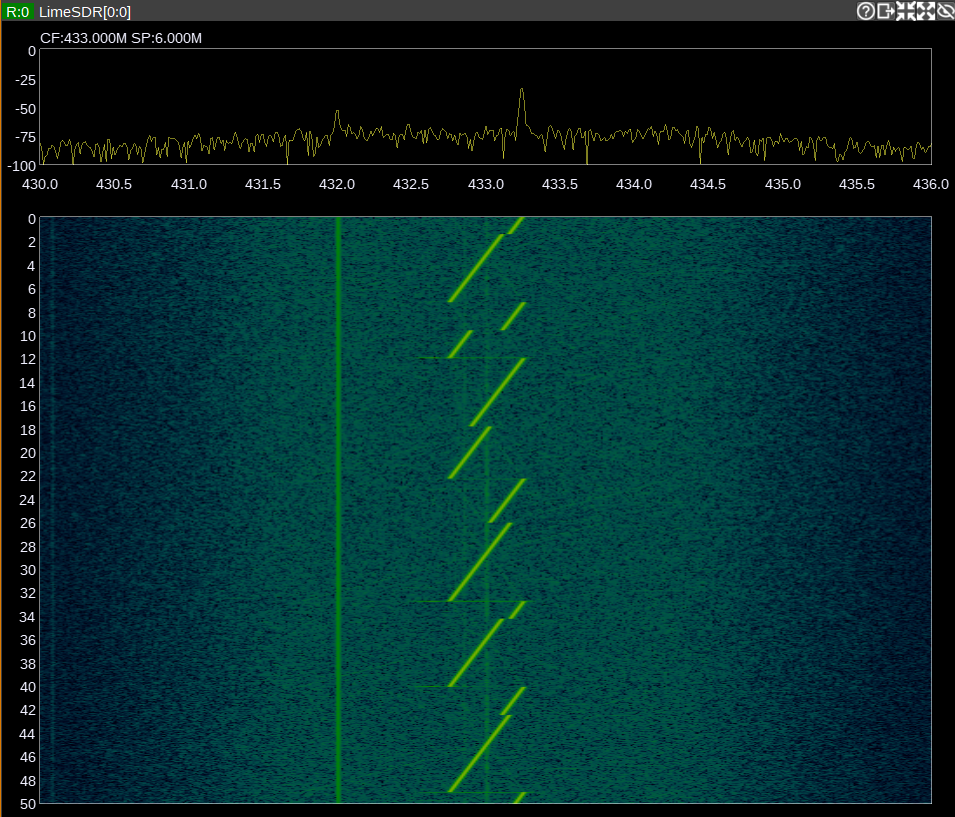
\includegraphics[width=0.8\linewidth]{../Images/loraValidationWithSDR.png}
    \caption{SDR Output for LoRa Transmission}
    \label{fig:loravalidationwithsdr}
\end{figure}

\subsection{Receiver Validation}
The receiver was deemed to be working properly after a test was performed to receive LoRa transmissions in mode 3, and the receiver successfully did that. The output of the receiver circuit can be seen in figure \ref{fig:receiveroutinvalidationtest} below.
\begin{figure}[H]
    \centering
    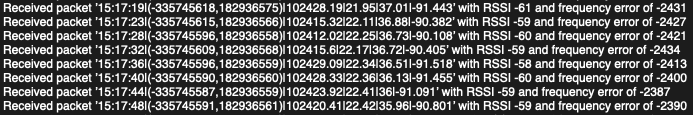
\includegraphics[width=1.0\linewidth]{../Images/receiverValidation.png}
    \caption{Receiver Output}
    \label{fig:receiveroutinvalidationtest}
\end{figure}
An interesting aspect of this above transmission to note is the fact that some frequency drift was experienced, indicated by the "frequency error" parameter. This frequency drift was related to the temperature differential between the transmission circuit and the receiver circuit LoRa modules. This frequency drift became an issue occasionally at the smaller bandwidth modes of operation due to those modes only being able to handle a frequency drift of roughly 10\% of the bandwidth of the mode of operation. When the frequency drift was more than this value, transmission errors were encountered. Due to this issue not actually causing too many errors, and the time that would have been lost in purchasing and implementing better temperature-compensated LoRa modules, the issue was ignored for the remainder of the testing process.
\section{Simulation}
The most important aspects of the project that I wanted to model, were the LoRa transmission protocols as described in section \ref{sec:loratransmissionparameters} of the literature review. It was important to gain an understanding of the preamble time, the payload time, and the total packet time for the various modes of operation of the system. Therefore, in table \ref{tab:simulationsymbolrateandtimeandlowdatarateoptimizationflag} below, the symbol rate ($R_{S}$), symbol time ($T_{S}$), and the low data rate optimisation flag have been calculated for all 60 modes of operation. The symbol rate and time are displayed in units of milliseconds. A note about the low data rate optimisation, while not mentioned often, this setting plays a crucial role in the  operation of the LoRa module. The low data rate optimisation register of the SX1278 must be set accordingly when the symbol time is greater than 16ms \cite{SX1278}. The symbol rate was calculated using equation \ref{eq:symbolrate}, and the symbol time was calculated using equation \ref{eq:symboltime}.

\begin{longtable}[H]{|c|c|c|c|c|c|}
\hline
Mode & \begin{tabular}[c]{@{}c@{}}Spreading\\ Factor\end{tabular} & \begin{tabular}[c]{@{}c@{}}Bandwidth\\ (kHz)\end{tabular} & \begin{tabular}[c]{@{}c@{}}Symbol Rate ($R_{S}$)\end{tabular} & \begin{tabular}[c]{@{}c@{}}Symbol Time ($T_{S}$)\end{tabular} & \begin{tabular}[c]{@{}c@{}}Low Data\\ Rate Optimisation\end{tabular} \\ \hline
1 & 7 & 7.8 & 60.94 & 16.41 & 1.00 \\ \hline
2 & 7 & 10.4 & 81.25 & 12.31 & 0.00 \\ \hline
3 & 7 & 15.6 & 121.88 & 8.21 & 0.00 \\ \hline
4 & 7 & 20.8 & 162.50 & 6.15 & 0.00 \\ \hline
5 & 7 & 31.25 & 244.14 & 4.10 & 0.00 \\ \hline
6 & 7 & 41.7 & 325.78 & 3.07 & 0.00 \\ \hline
7 & 7 & 62.5 & 488.28 & 2.05 & 0.00 \\ \hline
8 & 7 & 125 & 976.56 & 1.02 & 0.00 \\ \hline
9 & 7 & 250 & 1953.13 & 0.51 & 0.00 \\ \hline
10 & 7 & 500 & 3906.25 & 0.26 & 0.00 \\ \hline
11 & 8 & 7.8 & 30.47 & 32.82 & 1.00 \\ \hline
12 & 8 & 10.4 & 40.63 & 24.62 & 1.00 \\ \hline
13 & 8 & 15.6 & 60.94 & 16.41 & 1.00 \\ \hline
14 & 8 & 20.8 & 81.25 & 12.31 & 0.00 \\ \hline
15 & 8 & 31.25 & 122.07 & 8.19 & 0.00 \\ \hline
16 & 8 & 41.7 & 162.89 & 6.14 & 0.00 \\ \hline
17 & 8 & 62.5 & 244.14 & 4.10 & 0.00 \\ \hline
18 & 8 & 125 & 488.28 & 2.05 & 0.00 \\ \hline
19 & 8 & 250 & 976.56 & 1.02 & 0.00 \\ \hline
20 & 8 & 500 & 1953.13 & 0.51 & 0.00 \\ \hline
21 & 9 & 7.8 & 15.23 & 65.64 & 1.00 \\ \hline
22 & 9 & 10.4 & 20.31 & 49.23 & 1.00 \\ \hline
23 & 9 & 15.6 & 30.47 & 32.82 & 1.00 \\ \hline
24 & 9 & 20.8 & 40.63 & 24.62 & 1.00 \\ \hline
25 & 9 & 31.25 & 61.04 & 16.38 & 1.00 \\ \hline
26 & 9 & 41.7 & 81.45 & 12.28 & 0.00 \\ \hline
27 & 9 & 62.5 & 122.07 & 8.19 & 0.00 \\ \hline
28 & 9 & 125 & 244.14 & 4.10 & 0.00 \\ \hline
29 & 9 & 250 & 488.28 & 2.05 & 0.00 \\ \hline
30 & 9 & 500 & 976.56 & 1.02 & 0.00 \\ \hline
31 & 10 & 7.8 & 7.62 & 131.28 & 1.00 \\ \hline
32 & 10 & 10.4 & 10.16 & 98.46 & 1.00 \\ \hline
33 & 10 & 15.6 & 15.23 & 65.64 & 1.00 \\ \hline
34 & 10 & 20.8 & 20.31 & 49.23 & 1.00 \\ \hline
35 & 10 & 31.25 & 30.52 & 32.77 & 1.00 \\ \hline
36 & 10 & 41.7 & 40.72 & 24.56 & 1.00 \\ \hline
37 & 10 & 62.5 & 61.04 & 16.38 & 1.00 \\ \hline
38 & 10 & 125 & 122.07 & 8.19 & 0.00 \\ \hline
39 & 10 & 250 & 244.14 & 4.10 & 0.00 \\ \hline
40 & 10 & 500 & 488.28 & 2.05 & 0.00 \\ \hline
41 & 11 & 7.8 & 3.81 & 262.56 & 1.00 \\ \hline
42 & 11 & 10.4 & 5.08 & 196.92 & 1.00 \\ \hline
43 & 11 & 15.6 & 7.62 & 131.28 & 1.00 \\ \hline
44 & 11 & 20.8 & 10.16 & 98.46 & 1.00 \\ \hline
45 & 11 & 31.25 & 15.26 & 65.54 & 1.00 \\ \hline
46 & 11 & 41.7 & 20.36 & 49.11 & 1.00 \\ \hline
47 & 11 & 62.5 & 30.52 & 32.77 & 1.00 \\ \hline
48 & 11 & 125 & 61.04 & 16.38 & 1.00 \\ \hline
49 & 11 & 250 & 122.07 & 8.19 & 0.00 \\ \hline
50 & 11 & 500 & 244.14 & 4.10 & 0.00 \\ \hline
51 & 12 & 7.8 & 1.90 & 525.13 & 1.00 \\ \hline
52 & 12 & 10.4 & 2.54 & 393.85 & 1.00 \\ \hline
53 & 12 & 15.6 & 3.81 & 262.56 & 1.00 \\ \hline
54 & 12 & 20.8 & 5.08 & 196.92 & 1.00 \\ \hline
55 & 12 & 31.25 & 7.63 & 131.07 & 1.00 \\ \hline
56 & 12 & 41.7 & 10.18 & 98.23 & 1.00 \\ \hline
57 & 12 & 62.5 & 15.26 & 65.54 & 1.00 \\ \hline
58 & 12 & 125 & 30.52 & 32.77 & 1.00 \\ \hline
59 & 12 & 250 & 61.04 & 16.38 & 1.00 \\ \hline
60 & 12 & 500 & 122.07 & 8.19 & 0.00 \\ \hline
\caption{Simulation of symbol rate and time and low data rate optimisation flag}
\label{tab:simulationsymbolrateandtimeandlowdatarateoptimizationflag}
\end{longtable}

Once the symbol rate and time, and the low data rate optimisation flag were calculated, it then became possible to calculate the preamble using equation \ref{eq:preambletime}, the payload time using equation \ref{eq:payloadtimefinal}, and the packet time using equation \ref{eq:packettime}. It must be noted that to perform the payload time calculations, the following parameters were used; the payload size PL was set to the maximum size of a possible transmission for the system, which is 61 bytes, the CRC was set to 1 to indicate that the cyclic redundancy check was on, IH was set to 0 to indicate a header was present, and the coding rate CR was set to 1 which indicates a coding rate of 4/5 which was the designated coding rate for all testing.

\begin{longtable}[H]{|c|c|c|c|c|}
\hline
Mode & Preamble Time (ms) & Payload Size (bytes) & Payload Time (ms) & Packet Time (ms) \\ \hline
1 & 201.03 & 61.00 & 2264.62 & 2465.64 \\ \hline
2 & 150.77 & 61.00 & 1206.15 & 1356.92 \\ \hline
3 & 100.51 & 61.00 & 804.10 & 904.62 \\ \hline
4 & 75.38 & 61.00 & 603.08 & 678.46 \\ \hline
5 & 50.18 & 61.00 & 401.41 & 451.58 \\ \hline
6 & 37.60 & 61.00 & 300.82 & 338.42 \\ \hline
7 & 25.09 & 61.00 & 200.70 & 225.79 \\ \hline
8 & 12.54 & 61.00 & 100.35 & 112.90 \\ \hline
9 & 6.27 & 61.00 & 50.18 & 56.45 \\ \hline
10 & 3.14 & 61.00 & 25.09 & 28.22 \\ \hline
11 & 402.05 & 61.00 & 3708.72 & 4110.77 \\ \hline
12 & 301.54 & 61.00 & 2781.54 & 3083.08 \\ \hline
13 & 201.03 & 61.00 & 1854.36 & 2055.38 \\ \hline
14 & 150.77 & 61.00 & 1083.08 & 1233.85 \\ \hline
15 & 100.35 & 61.00 & 720.90 & 821.25 \\ \hline
16 & 75.20 & 61.00 & 540.24 & 615.44 \\ \hline
17 & 50.18 & 61.00 & 360.45 & 410.62 \\ \hline
18 & 25.09 & 61.00 & 180.22 & 205.31 \\ \hline
19 & 12.54 & 61.00 & 90.11 & 102.66 \\ \hline
20 & 6.27 & 61.00 & 45.06 & 51.33 \\ \hline
21 & 804.10 & 61.00 & 6432.82 & 7236.92 \\ \hline
22 & 603.08 & 61.00 & 4824.62 & 5427.69 \\ \hline
23 & 402.05 & 61.00 & 3216.41 & 3618.46 \\ \hline
24 & 301.54 & 61.00 & 2412.31 & 2713.85 \\ \hline
25 & 200.70 & 61.00 & 1605.63 & 1806.34 \\ \hline
26 & 150.41 & 61.00 & 957.70 & 1108.11 \\ \hline
27 & 100.35 & 61.00 & 638.98 & 739.33 \\ \hline
28 & 50.18 & 61.00 & 319.49 & 369.66 \\ \hline
29 & 25.09 & 61.00 & 159.74 & 184.83 \\ \hline
30 & 12.54 & 61.00 & 79.87 & 92.42 \\ \hline
31 & 1608.21 & 61.00 & 11552.82 & 13161.03 \\ \hline
32 & 1206.15 & 61.00 & 8664.62 & 9870.77 \\ \hline
33 & 804.10 & 61.00 & 5776.41 & 6580.51 \\ \hline
34 & 603.08 & 61.00 & 4332.31 & 4935.38 \\ \hline
35 & 401.41 & 61.00 & 2883.58 & 3284.99 \\ \hline
36 & 300.82 & 61.00 & 2160.96 & 2461.77 \\ \hline
37 & 200.70 & 61.00 & 1441.79 & 1642.50 \\ \hline
38 & 100.35 & 61.00 & 598.02 & 698.37 \\ \hline
39 & 50.18 & 61.00 & 299.01 & 349.18 \\ \hline
40 & 25.09 & 61.00 & 149.50 & 174.59 \\ \hline
41 & 3216.41 & 61.00 & 20480.00 & 23696.41 \\ \hline
42 & 2412.31 & 61.00 & 15360.00 & 17772.31 \\ \hline
43 & 1608.21 & 61.00 & 10240.00 & 11848.21 \\ \hline
44 & 1206.15 & 61.00 & 7680.00 & 8886.15 \\ \hline
45 & 802.82 & 61.00 & 5111.81 & 5914.62 \\ \hline
46 & 601.63 & 61.00 & 3830.79 & 4432.42 \\ \hline
47 & 401.41 & 61.00 & 2555.90 & 2957.31 \\ \hline
48 & 200.70 & 61.00 & 1277.95 & 1478.66 \\ \hline
49 & 100.35 & 61.00 & 557.06 & 657.41 \\ \hline
50 & 50.18 & 61.00 & 278.53 & 328.70 \\ \hline
51 & 6432.82 & 61.00 & 38334.36 & 44767.18 \\ \hline
52 & 4824.62 & 61.00 & 28750.77 & 33575.38 \\ \hline
53 & 3216.41 & 61.00 & 19167.18 & 22383.59 \\ \hline
54 & 2412.31 & 61.00 & 14375.38 & 16787.69 \\ \hline
55 & 1605.63 & 61.00 & 9568.26 & 11173.89 \\ \hline
56 & 1203.26 & 61.00 & 7170.46 & 8373.72 \\ \hline
57 & 802.82 & 61.00 & 4784.13 & 5586.94 \\ \hline
58 & 401.41 & 61.00 & 2392.06 & 2793.47 \\ \hline
59 & 200.70 & 61.00 & 1196.03 & 1396.74 \\ \hline
60 & 100.35 & 61.00 & 516.10 & 616.45 \\ \hline
\caption{Simulation of preamble, payload, and packet time}
\label{tab:simulationofpreamblepayloadandpackettime}
\end{longtable}

One can see from table \ref{tab:simulationofpreamblepayloadandpackettime} that as the bandwidth for each spreading factor is increased, then the packet time decreases. One can also begin to understand why LoRa is defined as a low bitrate communication protocol, because for some of the modes, to fully transmit a 61-byte payload packet, it can take upwards of 30 seconds, like in mode 51.
% ----------------------------------------------------
\ifstandalone
\bibliography{../Bibliography/References}
\printnoidxglossary[type=\acronymtype,nonumberlist]
\fi
\end{document}
% ----------------------------------------------------